\documentclass[../main.tex]{subfiles}
\begin{document}
\chapter{Forbruger} \label{Chap:Forbruger}

\section{Boost Konverter}
Der skal implementeres en Step-up/boost converter efter Energilagret så der kan outputtes en højere og stabil ønsket spænding end hvad energilageret selv kan generere. Ifølge kravspecifikationen skulle der leveres 10 volt til en load. 

\subsection{Kontrollering}
Kontrolleren er den samme som i Buck Konverteren fra Kraftværk sektionen, bare med et par linjer lavet om. Den sørgede dermed at outputtet til loadet altid var 10V.

\section{Belastning}

\section{Test}
Følgende kravspecifikationer tilhører denne del af projektet
\begin{enumerate}
  \item Spændingen V2 skal være indenfor +/- 1.0 volt
  \item Spændingskilde V2 skal kunne levere min. 150 mA.
  \item Spændingen V2 skal være indenfor +/- 1.0 volt ved en belastningsændring fra 50 mA til 150 mA indenfor 1.0 s.
\end{enumerate}

For at teste Krav 4, belaster vi udgangen af boost konverteren med en tilfældig load og målte spændingen over den. Det kan ses på Figur \ref{fig: Krav 4 Opfyldt} at spændingen (grøn) er 9.91V, og kravet dermed er overholdt.
\begin{figure}[H]
      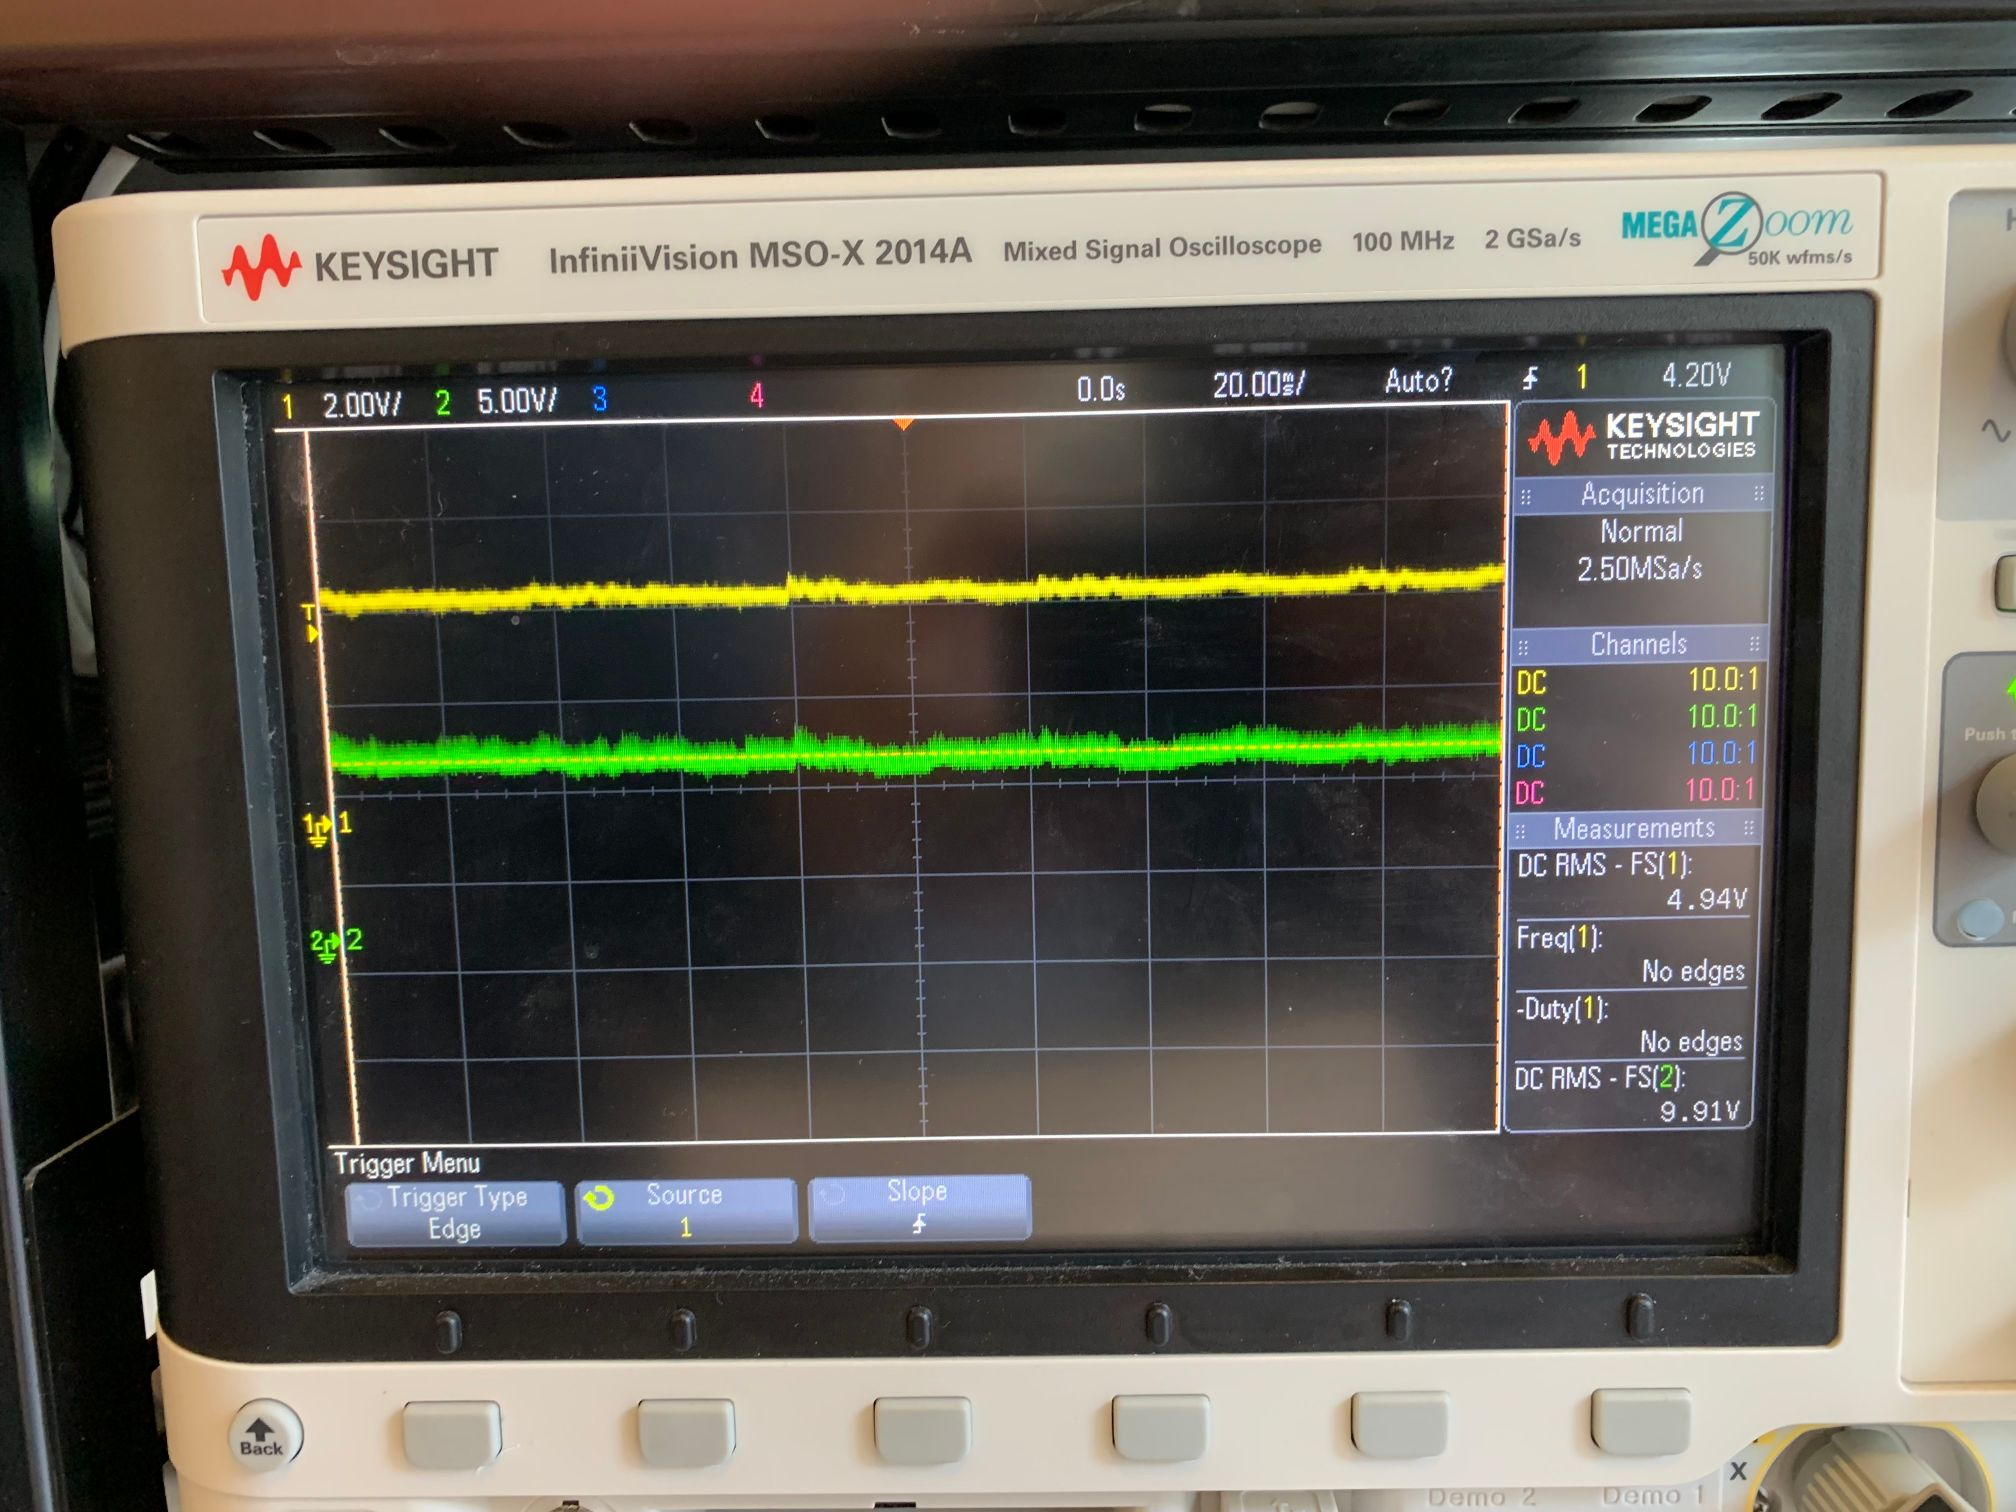
\includegraphics[width=\textwidth]{Dokumentation/Pictures/Krav4.jpg}
     \caption{Krav 4 Opfyldt}
     \label{fig: Krav 4 Opfyldt}
     \end{figure}

For at teste Krav 5, belaster vi udgangen af buck konverteren (4.8V) med 5$\Omega$ hvilket svarer til nogenlunde 300mA ved 15V. Det kan ses på Figur \ref{fig: Krav 5 og 6 Opfyldt} at spændingen er 14.9V, og kravet dermed er overholdt.

For at teste Krav 6, belaster vi udgangen af buck konverteren (4.8V) med 5$\Omega$ og skifter den derefter hurtigt til 164$\Omega$ hvilket svarer til nogenlunde at hoppe fra 100mA til 300mA ved 15V. Det kan ses på Figur \ref{fig: Krav 5 og 6 Opfyldt} at spændingen er -1V efter 1 sekund, og kravet dermed er overholdt.

\begin{figure}[H]
      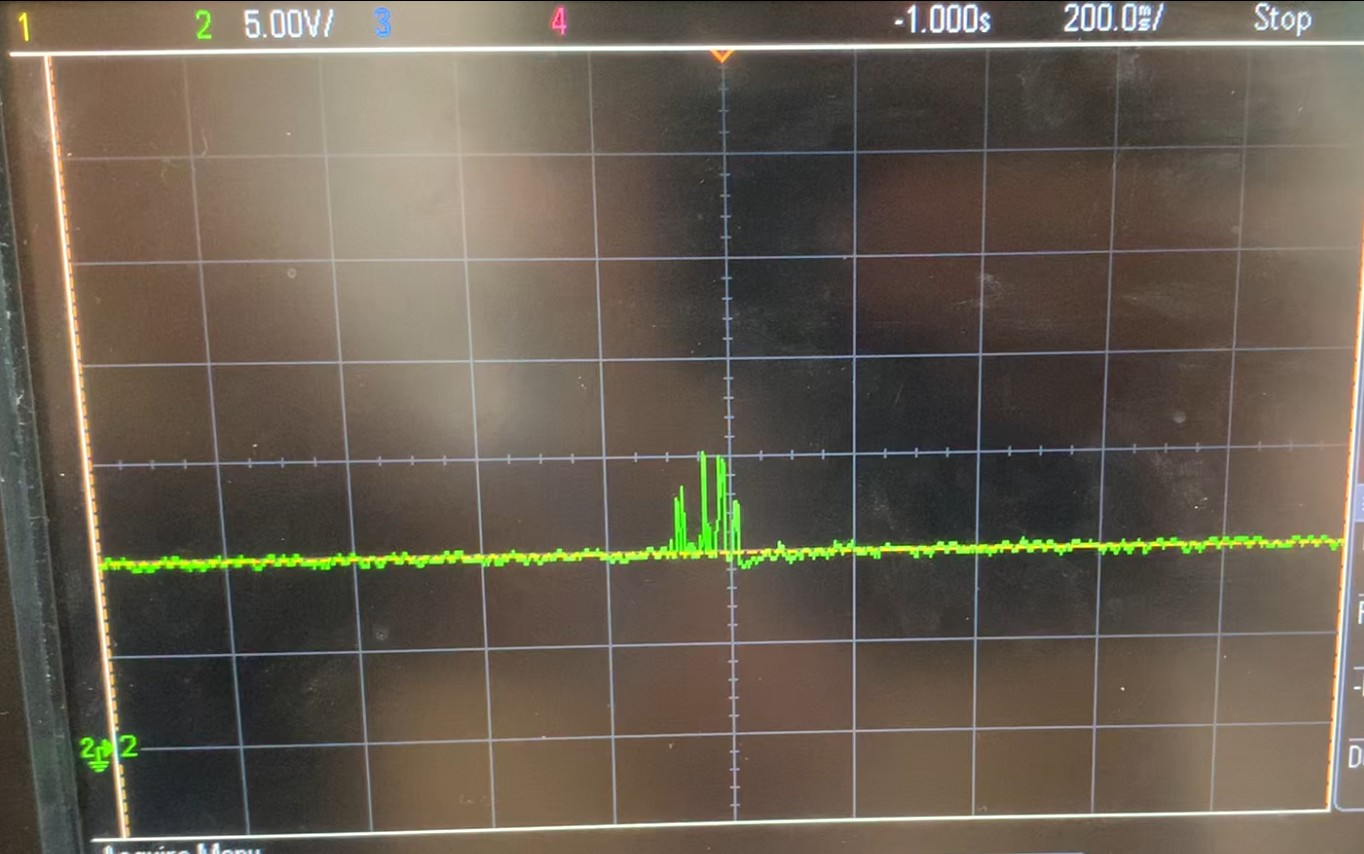
\includegraphics[width=\textwidth]{Dokumentation/Pictures/Krav5og6.jpg}
     \caption{Krav 5 og 6 Opfyldt}
     \label{fig: Krav 5 og 6 Opfyldt}
     \end{figure}

De tre krav er allesammen overholdt, og testen er dermed en succes. 

\end{document}